\chapter{The CMS Detector}
\label{chap:detector}

The detector is cylindrically symmetric, with a modular design consisting of different subsystems specialized for detection or identification of specific particles. Many of the Standard Model particles are unstable. In fact only about 8 particles are directly detected in our experiment, the rest of those being reconstructed via their decay into these more stable elements. Of all the Standard Model particles, 

Figure \ref{fig:howcmsworks} is a depiction of the CMS detector. Figure \ref{fig:schematicview} is a schematic view of the CMS detector and the particles it interacts with.

\begin{figure}[htbp]
\centering
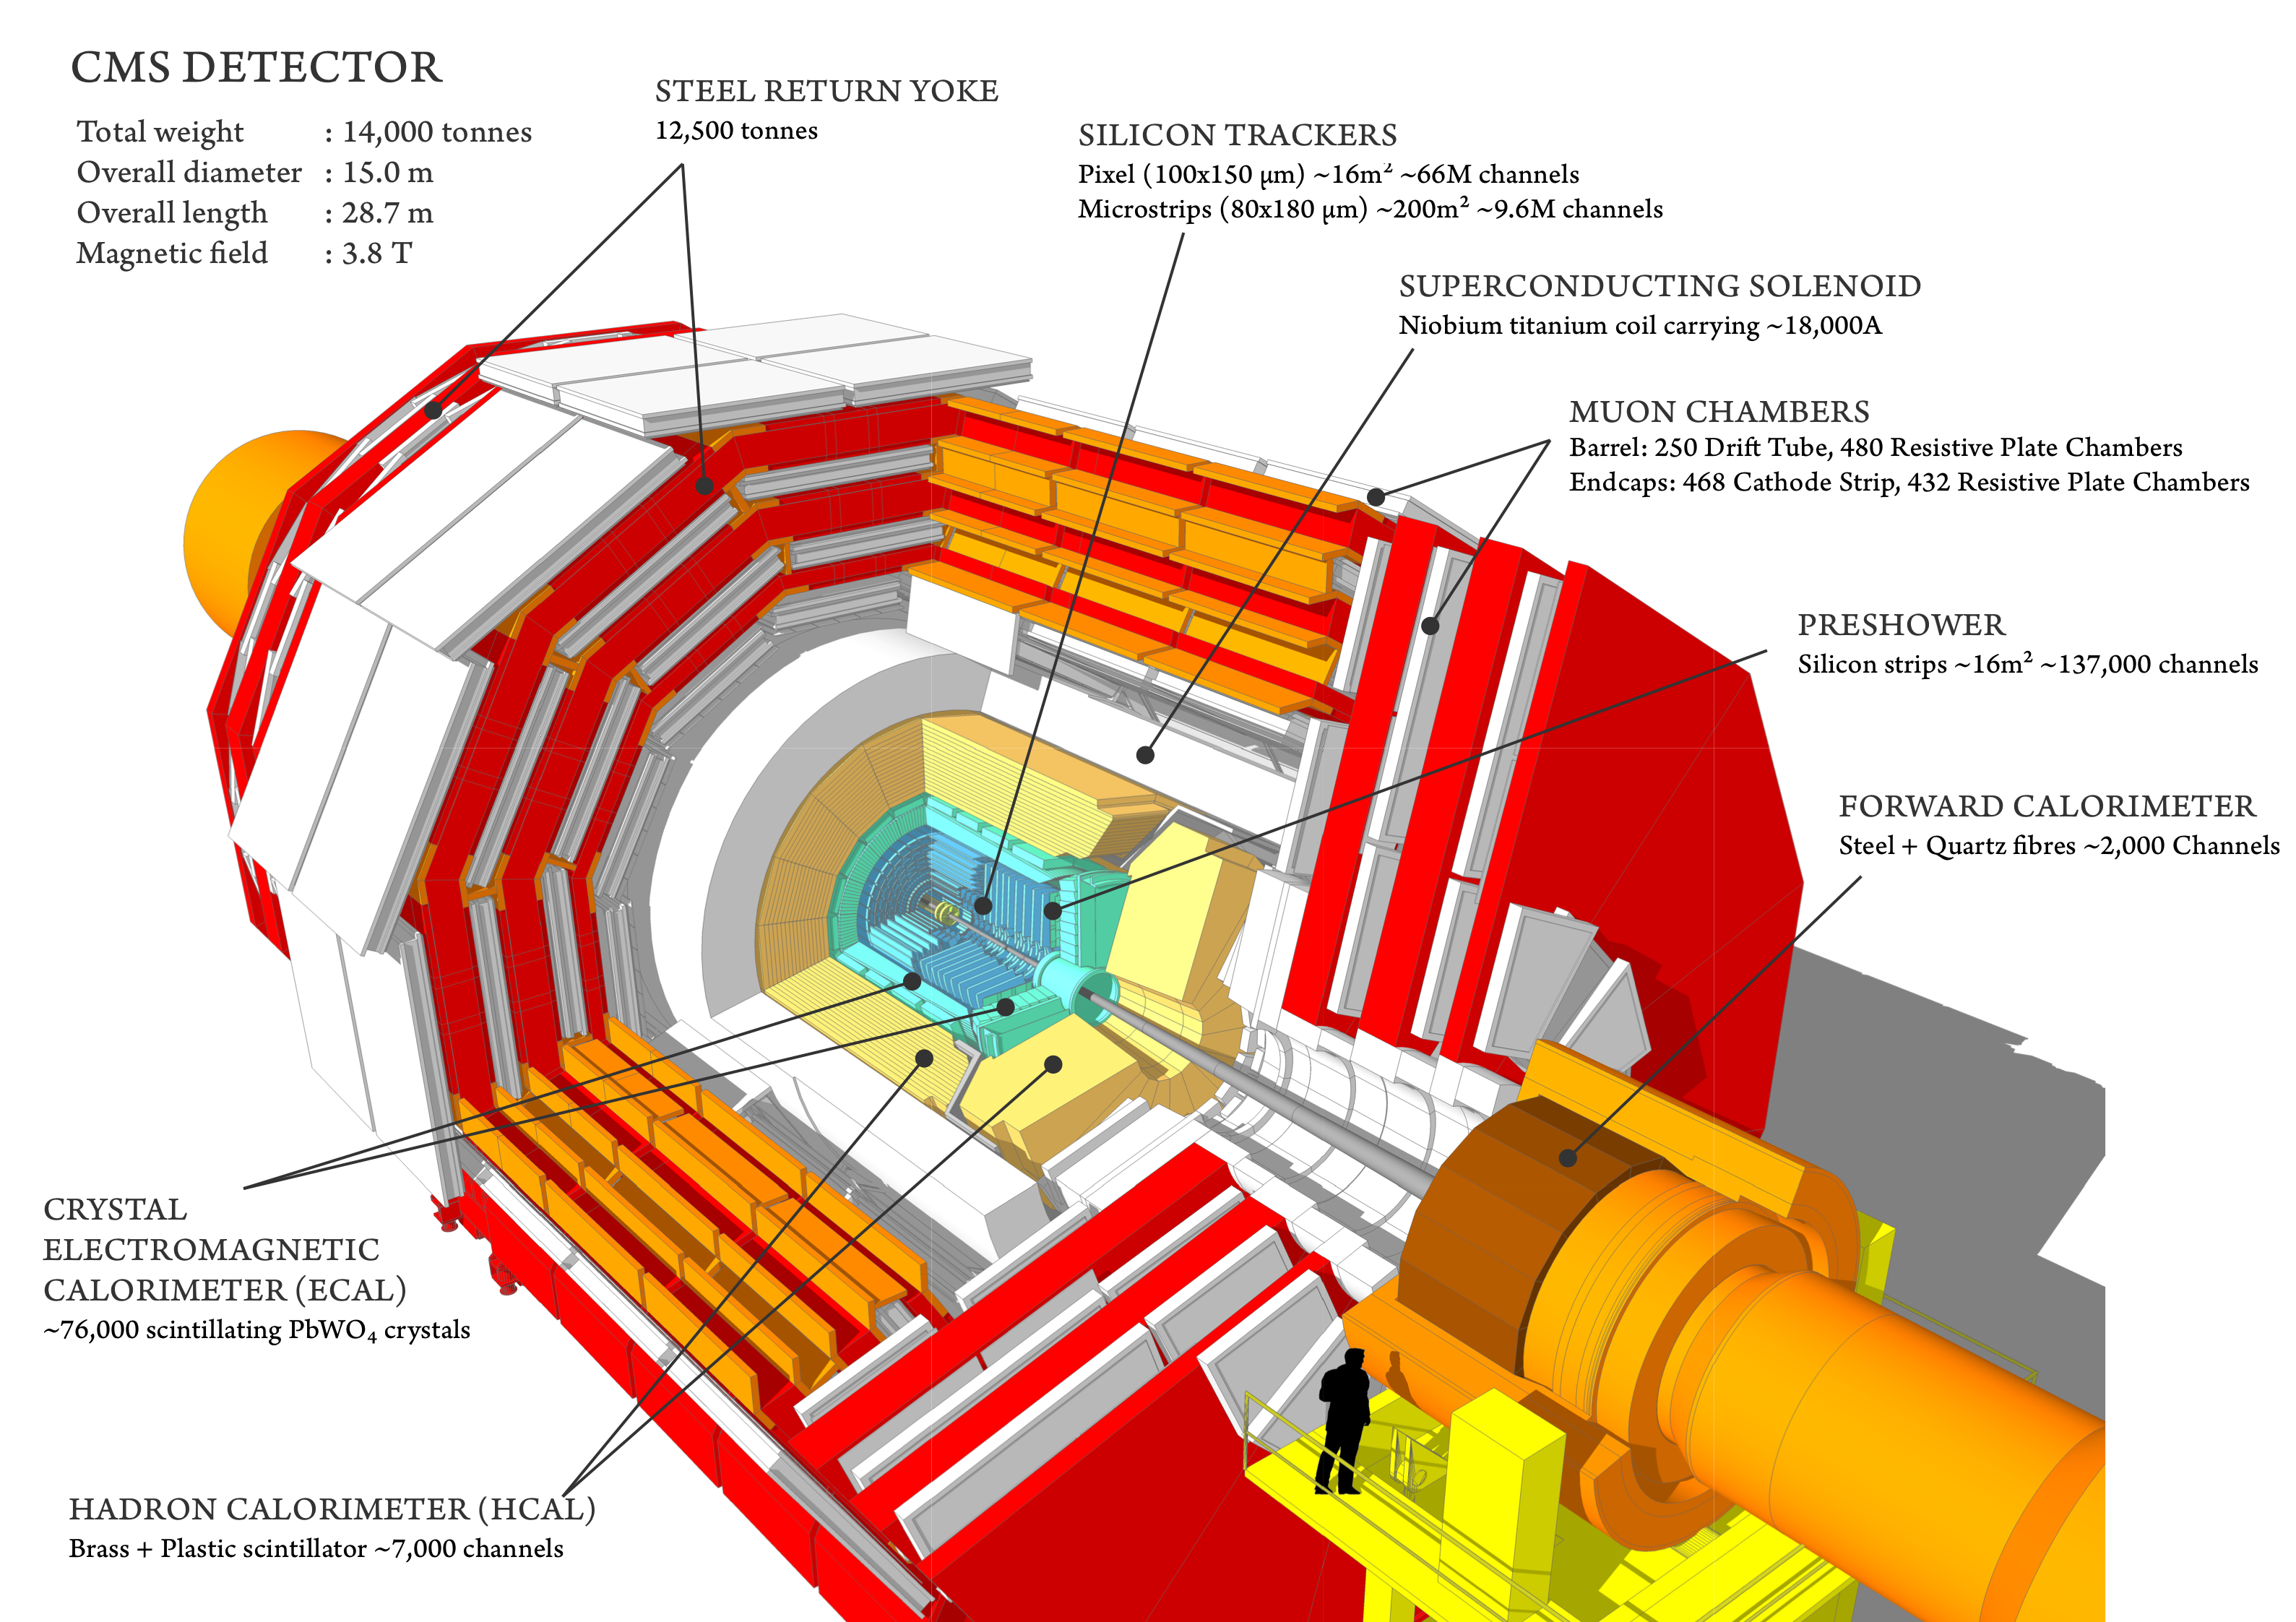
\includegraphics[width=90mm]{figs/howcmsworks.png}
\caption{A depiction of the CMS detector.}
\label{fig:howcmsworks}
\end{figure}

\begin{figure}[htbp]
\centering
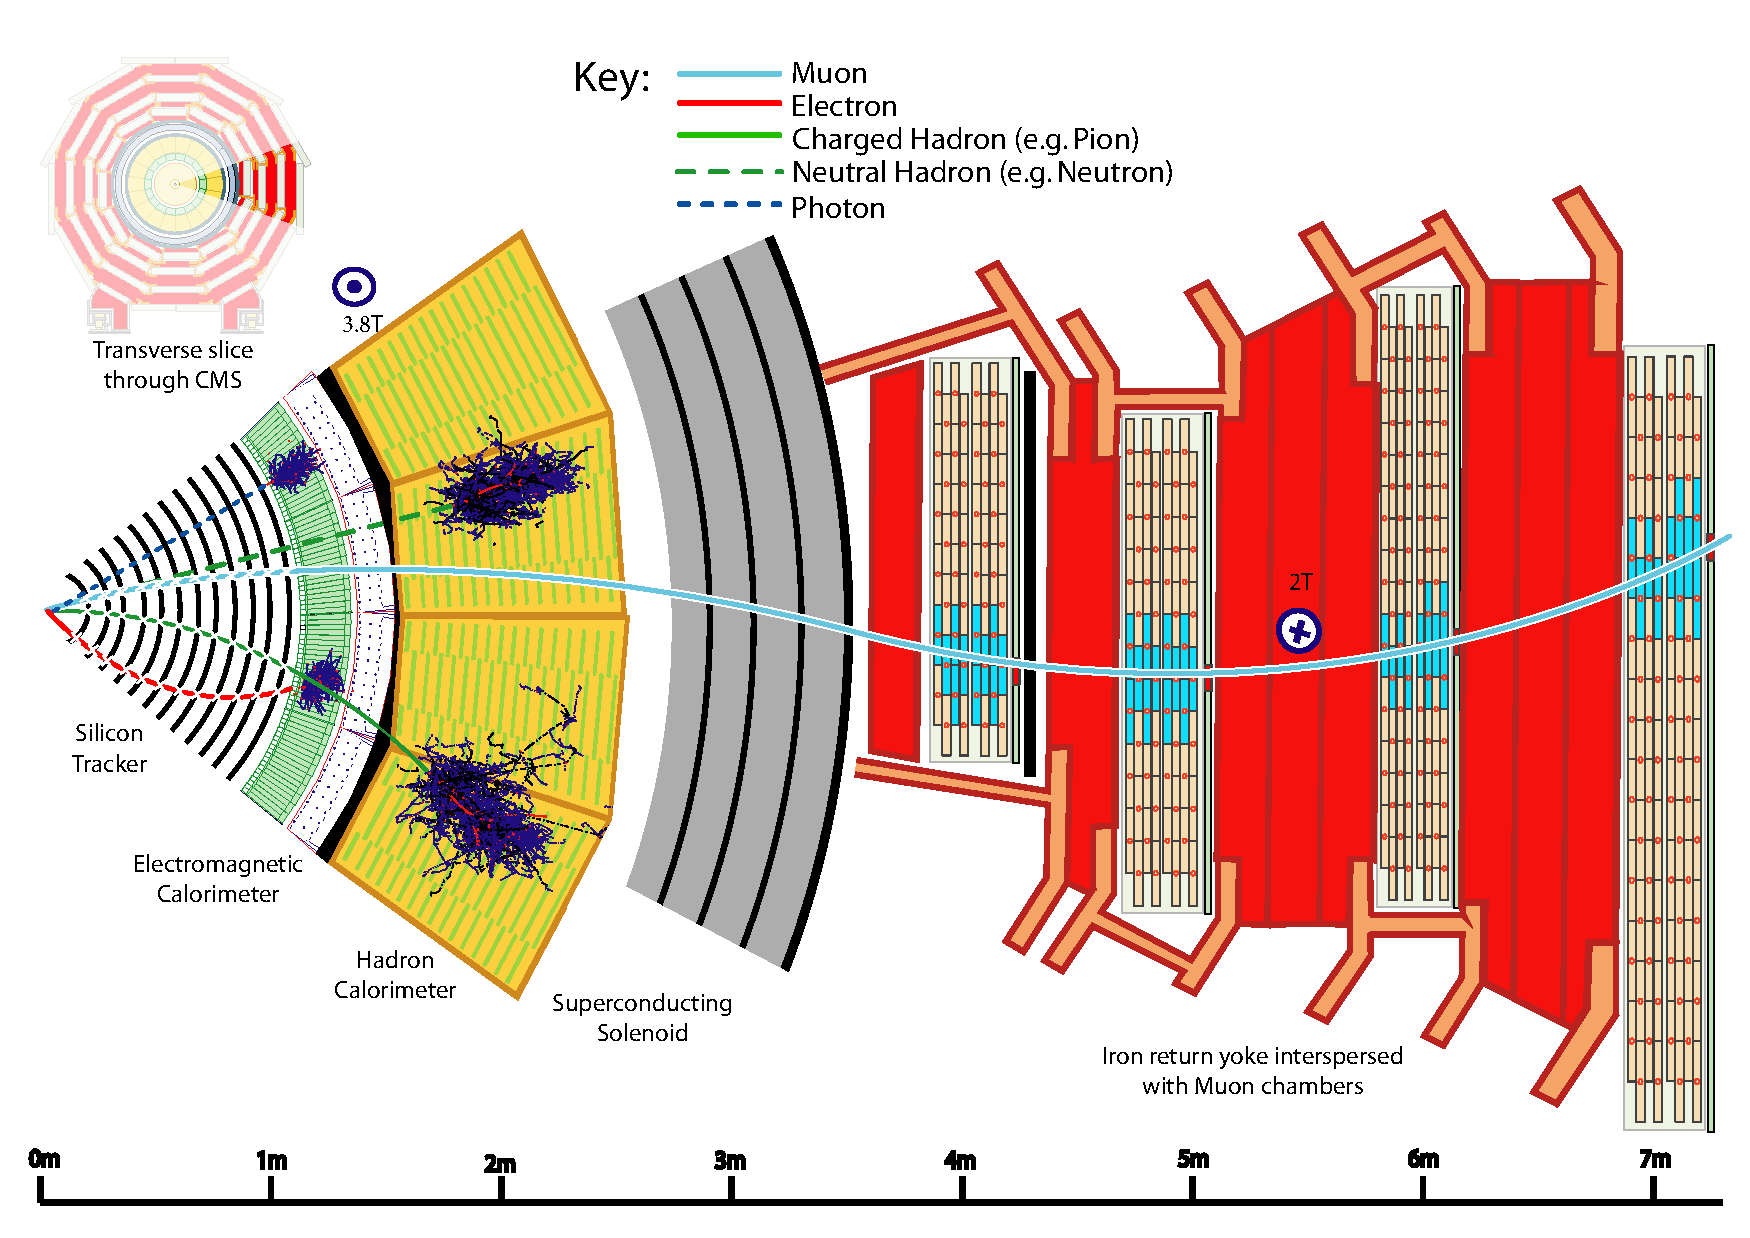
\includegraphics[width=90mm]{figs/CMS-PRF-14-001_Figure_001.pdf}
\caption{A schematic view of the CMS detector and the particles it interacts with.}
\label{fig:schematicview}
\end{figure}

\section{Silicon Tracker}
At the center of the detector lies the silicon tracker which is responsible for momentum reconstruction of charged particles and reconstruction of the primary vertices created from a proton-proton interaction. The tracker is composed of a number of concentric cylindrical layers each instrumented with silicon sensors. As a charged particle traverses an individual sensor a small amount of ionization energy is deposited in that element. A bias voltage is applied across the sensor to direct the charge to either end of the sensor. Bonded to the sensors are front-end electronics responsible for the amplification and shaping of the resultant signal. Neighboring elements are clustered together creating what is known as a ``hit''. These hits are then used to reconstruct the particle's trajectory through the tracker. To make a measurement of the momentum and charge of the particle, the tracker is immersed in a 3.8 T magnetic field which bends the trajectory of the particle.

The tracker is further divided into an inner and outer parts which make use of slightly different technologies. The inner part of the tracker is known as the pixel detector and consists of 4 layers which the sensitive elements are silicon pixels of size 100x150 $\mu$m. This fine granularity of

\section{Electromagnetic Calorimeter}
\section{Hadronic Calorimeter}
\section{Solenoidal Magnet}
\section{Muon System}
\section{Particle Flow Event Reconstruction}

Particle Flow event reconstruction is pretty good.\cite{CMS-PRF-14-001}
\section{Trigger System}
